% Затехал Иваныч
\documentclass[../main.tex]{subfiles}
\begin{document}

\section{Билет 4. Смешанная задача для колебаний полубесконечной струны с закрепленным концом. Условия согласования начальных и граничного данных. Существование и единственность классического решения.}

\subsection{Формулировка}

Задача (называется \emph{начально-краевой} или \emph{смешанной})
\begin{equation} \label{4_1}
\begin{cases}
  u_{tt} -a^2u_{xx} = 0 ,\;\;\, t>0,\; x>0 \\
  \begin{aligned}
    \while{u}{t=0}\; &= u_0(x),\quad x\geq 0 \\
    \while{u_t}{t=0} &= u_1(x),\quad x\geq 0  \\
    \while{u}{x=0} &= 0, \;\; \text{по сравнению с задачей Коши это дополнительное граничное условие}
  \end{aligned}
\end{cases}
\end{equation}
\vspace{0pt}  % Почему-то это создаёт дополнительный отступ, которого не хватало

\begin{remark}
    Физический смысл: смотрим, как волна отражается от закрепленного конца  
\end{remark}
Предполагаем, что 
\begin{equation*}
    \begin{cases}
        u_0(x) \in C^2 [0, +\infty) \\
        u_1(x) \in C^1 [0, +\infty) \\
    \end{cases}
\end{equation*}

\subsection{Общее решение}

\begin{align*}
&\ \ u(t,x) = f(x +at) + g(x - at) \\
&\begin{cases}
  \begin{aligned}
    \while{u}{t=0}\; &= f(x) + g(x) = u_0(x), \;\; &x \geq 0\\
    \while{u_t}{t=0} &= af'(x) -ag'(x) = u_1(x), \;\; &x \geq 0  
  \end{aligned}
\end{cases}
\end{align*}
Если ввести обозначение $v_1 = \displaystyle\int_0^x u_1(y)\;dy + C$, то при $x \geq 0$

\begin{wrapfigure}[7]{r}{0.35\textwidth}
    \centering
    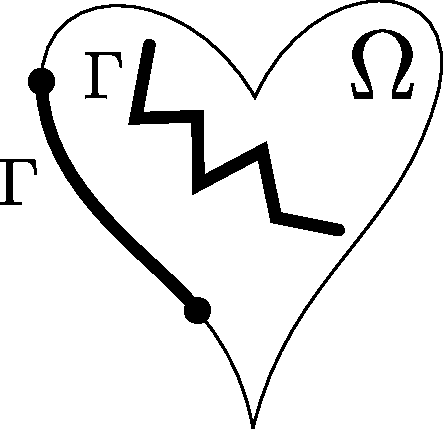
\includegraphics[width=0.35\textwidth]{./pic 4_1.pdf}
\end{wrapfigure}

\begin{align*}
    & f(x) = \frac{1}{2}u_0(x) + \frac{1}{2a}v_1(x) \\
    & g(x) = \frac{1}{2}u_0(x) - \frac{1}{2a}v_1(x) \\
\end{align*}

Граничные условия нужны для определения $u$ в $(x \geq 0)\cap(t \geq 0)$ (в смысле пересечения областей). Их не обязательно ставить на $x=0$, можно на $x + \alpha t = 0, \; -a < \alpha < a$, то есть там, где известна только одна из функций, а не обе.
$$
\while{u}{x=0} = f(at) + g(-at)=0, \;\; t \geq 0
$$
\clearpage % костыль чтобы wrapfigure не думал, что иллюстрация простирается на следующие страницы тоже

\begin{wrapfigure}[7]{r}{0.35\textwidth}
    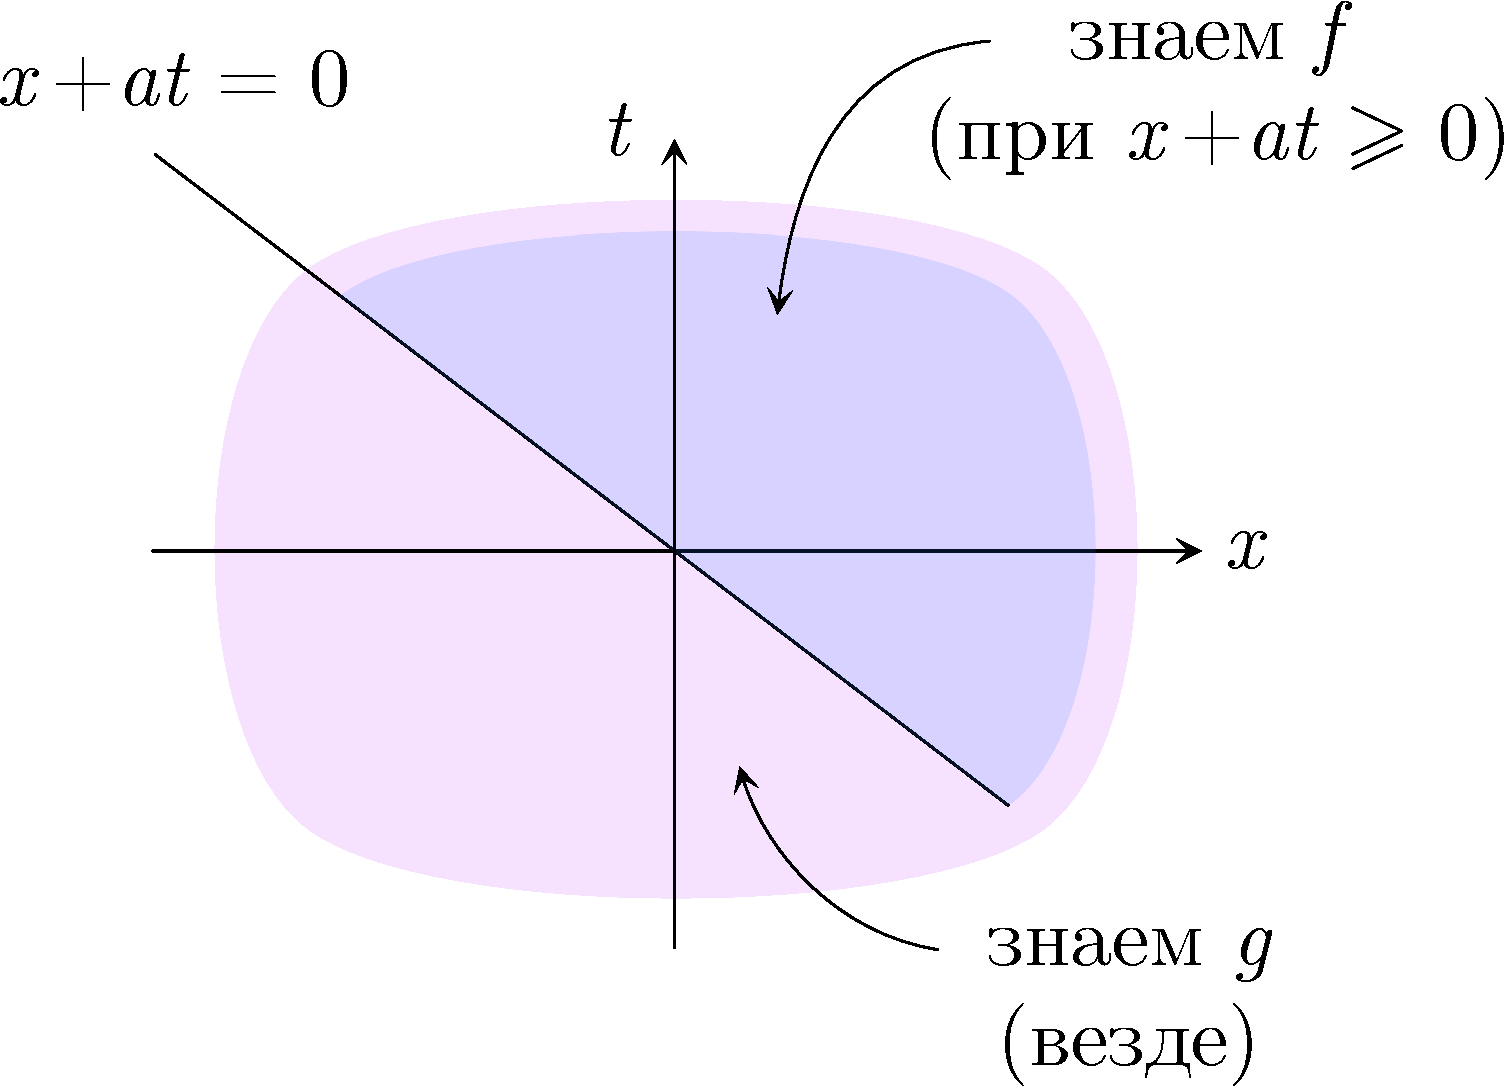
\includegraphics[width=0.35\textwidth]{./pic 4_2.pdf}
\end{wrapfigure}

Введем $\xi = -at, \xi \leq 0$, тогда $g(\xi) = -f(-\xi)$ и суммарно:
\begin{equation*}
    g(\xi) = \begin{cases}
        \frac{1}{2}u_0(\xi)-\frac{1}{2a}v_1(\xi), & \xi \geq 0\\
        -\frac{1}{2}u_0(-\xi)-\frac{1}{2a}v_1(-\xi), & \xi \leq 0\\
    \end{cases}
\end{equation*}

Теперь $g$ известна везде, решение найдено при $x + at > 0$, то есть даже в большей области, чем мы хотели.


\subsection{Сшивка}
Чтобы $g(x) \in C^2(\R)$, решения необходимо <<сшить>>
\begin{align*}
    g(+0) &= g(-0) \\
    g'(+0) &= g'(-0) \\
    g''(+0) &= g''(-0)
\end{align*}
Распишем эти условия:
\begin{align*}
     g(+0) &= g(-0) &\Leftrightarrow&& 
    \frac{1}{2}u_0(0) - \cancel{\frac{1}{2a}v_1(0)} &= -\frac{1}{2}u_0(0) - \cancel{\frac{1}{2a}v_1(0)} &&\Rightarrow& u_0(0) &= 0 \\
     g'(+0) &= g'(-0) &\Leftrightarrow&& \cancel{\frac{1}{2}u'_0(0)} - \frac{1}{2a}u_1(0) &=
    \cancel{\frac{1}{2}u'_0(0)} + \frac{1}{2a}u_1(0) &&\Rightarrow& u_1(0) &= 0 \\
     g''(+0) &= g''(-0) &\Leftrightarrow&& \frac{1}{2} u''_0(0) - \frac{1}{2a} u_1'(0) &= -\frac{1}{2}u_0''(0) - \frac{1}{2a} u_1'(0) &&\Rightarrow& u_0''(0) &= 0
\end{align*}

\begin{definition}[условия согласования]
    Эти условия называются условиями согласования (начальных и граничных условий)
\end{definition}

При их выполнении решение будет классическим. Если $u_0(0) \ne 0$, то даже обобщенного решения не будет.

\subsection{Окончательное решение задачи}

\begin{equation} \label{4_2}
        u(t, x) = \begin{cases}
            \dfrac{u_0(x+at) + u_0(x-at)}{2} + \dfrac{1}{2a}\displaystyle\int_{x-at}^{x+at}u_1(y)\;dy,\quad & \{x\geq -at,\; x\geq at\} \\[1em]

            \dfrac{u_0(at+x) - u_0(at-x)}{2} + \dfrac{1}{2a}\displaystyle\int_{at-x}^{at+x}u_1(y)\;dy,\quad & \{x\geq -at,\; x\leq at\}
        \end{cases}
\end{equation}
\vspace{0pt}

\begin{theorem}
    Пусть в смешанной задаче \ref{4_1} функции $u_0(x)$ и $u_1(x)$ таковы, что 
    \begin{itemize}
        \item Выполнено условие гладкости: $u_0(x)\in \C^2[0, +\infty), \; u_1(x) \in \C^1[0, +\infty)$
        \item Выполнено условие согласования: $u_0(0) = u_1(0) = u_0''(0) = 0$
    \end{itemize}
    Тогда задача \ref{4_1} имеет единственное классическое решение $u(t,x) \in \C^2(t \geq 0, x\geq 0)$, представленное в \ref{4_2}
\end{theorem}

\begin{proof}
    Используем метод продолжений. Для задачи 
    $$
    \begin{cases}
        u_{tt} -a^2u_{xx} = 0, & t > 0,\; x > 0\\
        \while{u}{t=0} = u_0(x), & x \geq 0\\
        \while{u_t}{t=0} = u_1(x), & x \geq 0\\
        \while{u}{x=0} = 0, & t \geq 0
% у паши тут опечатка
    \end{cases}
    $$  
Введем
$$ \hat u_0(x) = 
\begin{cases}
    u_0(x), & x \geq 0 \\
    -u_0(-x), & x < 0
\end{cases} \qquad \hat u_1(x) = 
\begin{cases}
    u_1(x), & x \geq 0 \\
    -u_1(-x), & x < 0
\end{cases}
$$
Тогда 
$$
\begin{cases}
    \hat u_{tt} -a^2\hat u_{xx} = 0, & t > 0,\; x \in \R^1 \\
    \while{\hat u}{t=0} = \hat u_0(x), & x \in \R^1 \\
    \while{\hat u_t}{t=0} = \hat u_1(x), & x \in \R^1 \\
\end{cases} \; \text{ -- свели к задаче Коши}
$$
\vspace{0pt}

Решение дается формулой Даламбера:
$$
\hat u(t, x) = \frac{\hat u_0(x + at) + \hat u_0(x - at)}{2} +\frac{1}{2a}
\int_{x-at}^{x+at}\hat u_1(y)\;dy
$$

Покажем нечетность по $x$:
\begin{multline*}
\hat u(t, -x) = \frac{\hat u_0(-x + at) + \hat u_0(-x - at)}{2} +\frac{1}{2a}
\int_{-x-at}^{-x+at}\hat u_1(y)\;dy =
\frac{\hat u_0(x - at) + \hat u_0(x + at)}{2} -\\
-\frac{1}{2a}\int_{x-at}^{x+at}\hat u_1(y)\;dy = -\hat u(t, x)
\end{multline*}
\begin{multline*}
\hat u(t, 0) = \underbrace{\frac{\hat u_0(- at) + \hat u_0(at)}{2}}_{=0} + \frac{1}{2a} \int_{-at}^{+at} \hat u_1(y)\;dy = 0\hfill
\end{multline*}
\end{proof}
\end{document}